% Figure 7: learning controls. Rendered by render_tables.py via render_figures.figure7 from the v3
% contrasts, the matched v3 summary and the ablation summary; nothing numeric is typed here.
\begin{figure}[!htbp]
\centering
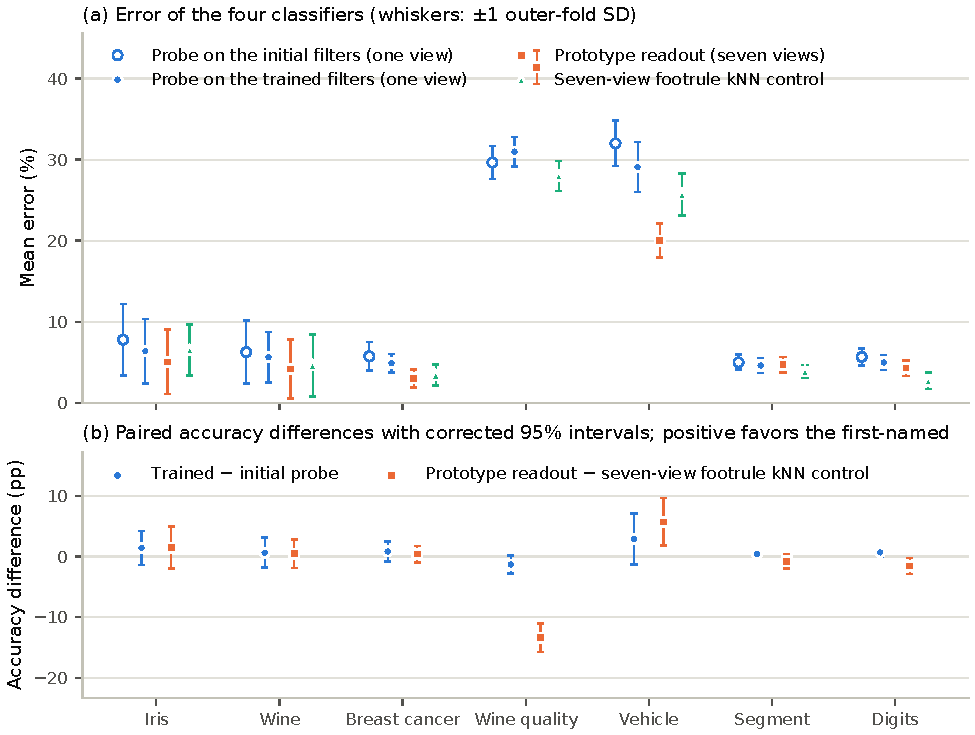
\includegraphics[width=\textwidth]{figures/data/fig7_learning_controls.pdf}
\caption{\textbf{Prototype-readout contrasts.} (a)~Mean outer-fold test error in percent on the seven benchmark datasets of four classifiers. A footrule kNN probe reads the hidden ranking of a single-view $[128]$ network before training (initial filters) and after training, with neighbor count and weighting chosen on inner folds (matched study). The others are the prototype readout with $K=7$ views and the seven-view footrule kNN control, footrule kNN on the same encoded views tuned on inner folds (component ablation). Whiskers are $\pm1$ outer-fold SD. (b)~The paired contrasts of Table~\ref{tab:contrasts}, trained minus initial probe and prototype readout minus kNN control, as accuracy differences in percentage points with 95\% corrected resampled-$t$ intervals (not simultaneous); positive favors the first-named. The prototype readout is at or above the kNN control on four datasets and below it on three. The trained probe is above the initial probe on six, and none of the seven probe intervals excludes zero. After Holm adjustment, one of the 14 contrasts remains significant (Wine quality prototype readout).}
\label{fig:learning-controls}
\end{figure}
